\documentclass{beamer}
%\documentclass[aspectratio=169]{beamer}
%
\mode<presentation>
{
  \usetheme{default}      
  \usecolortheme{default}
  \usefonttheme{default} 
  \setbeamertemplate{navigation symbols}{}
  \setbeamertemplate{caption}[numbered]
} 

\usepackage[english]{babel}
\usepackage[utf8x]{inputenc}

\title[Course presentation]{Introduction to machine learning course}
\subtitle{Lecture 1: Introduction and presentation of the course}
\author{Alexis Zubiolo\newline\texttt{alexis.zubiolo@gmail.com}}
\institute{Data Science Team Lead @ Adcash}
\date{\today}

\begin{document}

\begin{frame}
  \titlepage
\end{frame}

\begin{frame}{Before we start}
\vfill
I'd like to know a little bit more about you
\vfill
\begin{itemize}
	\item Short presentation: Name, occupation, \ldots
	\item Background in machine learning?
	\item Background in programming?
	\item Background in mathematics?
	\item Expectations from the course (if any)?
\end{itemize}
\vfill
Please send me an email so that I have your contact:
\vfill
\begin{center}
\texttt{alexis.zubiolo@gmail.com}
\end{center}
\vfill
All the material will be available on my personal GitHub:
\vfill
\begin{center}
\texttt{https://github.com/azubiolo/itstep}
\end{center}
\vfill
\end{frame}

\begin{frame}{Outline}
\vfill
\begin{itemize}
  \item What machine learning is, what it is not
\vfill
  \item A few practical examples
  \begin{itemize}
  	\item classification
  	\item regression
  \end{itemize}
\vfill
  \item Goals and presentation of the course 
\vfill
  \item Questions and answers
\end{itemize}
\vfill

\end{frame}

\begin{frame}{What is machine learning?}
\vfill
A simple example\ldots
\vfill
\begin{figure}
\centering
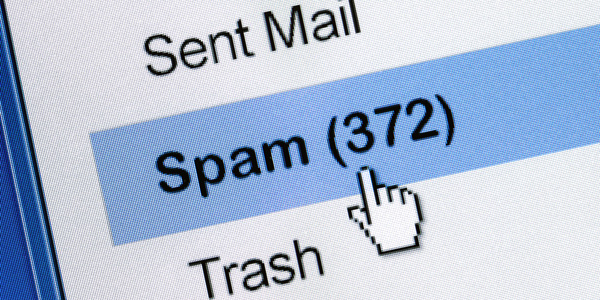
\includegraphics[width=\textwidth]{images/spam.jpg}
\end{figure}
\vfill
How to filter spam emails \textbf{automatically}?
\vfill
\end{frame}

\begin{frame}{Machine learning paradigm}
~\\
\vfill
Goal: Build algorithms that can 
\begin{itemize}
	\item \textbf{learn} from data
	\item \textbf{make predictions} on (new) data
\end{itemize}
\vfill
\pause
\begin{figure}
\centering
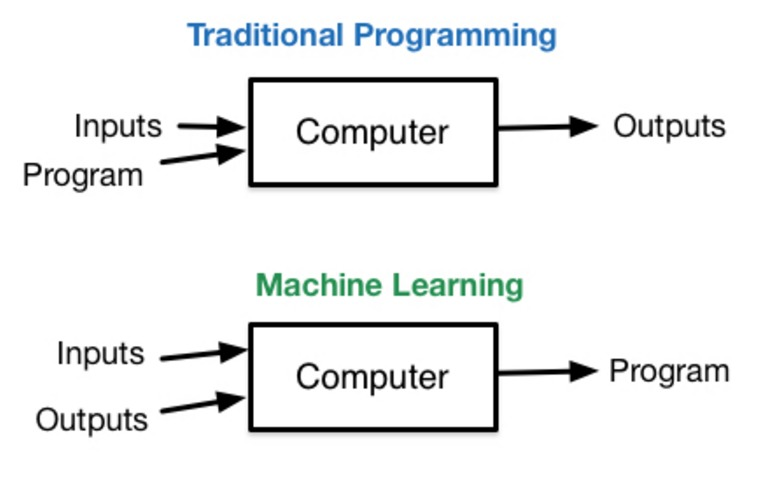
\includegraphics[width=\textwidth]{images/ml_vs_traditional.jpg}
\end{figure}
\vfill
\end{frame}

\begin{frame}{Main components of machine learning}

\vfill
Mathematics
\begin{itemize}
	\item Linear algebra
	\item Calculus
	\item Numerical optimization
\end{itemize}
\vfill
Statistics, probability theory
\vfill
Computer science
\vfill
I will assume some knowledge in computer science (= a language you are comfortable with). 
\vfill
\end{frame}

\begin{frame}{Example 1: Regression}

Regression = output is a \textbf{continuous} numerical value
\vfill
Example: \textbf{Estimate the price} of an apartment
\begin{itemize}
	\item input: \textbf{information} about the apartment
	\item output: \textbf{price}
\end{itemize}
\vfill
\pause
\begin{table}
\centering
\begin{tabular}{r|r}
living area (m$^2$) & price (1000's euros) \\\hline
50 & 30 \\
76 & 48 \\
26 & 12 \\
102 & 90 \\
\pause
61 & ?
\end{tabular}
\end{table}
\vfill
Linear model: price = \textbf{a} $\times$ area + \textbf{b}
\vfill
Problem: optimal values for \textbf{a} and \textbf{b}?

\end{frame}

\begin{frame}{Regression}

More data for a richer model:
\vfill
\begin{table}
\centering
\begin{tabular}{r|r|r}
living area (m$^2$) &  \textbf{\# bedrooms} & price (1000's euros) \\\hline
50 & \textbf{1} & 30\\
76 & \textbf{2} & 48\\
26 & \textbf{1} & 12\\
102 & \textbf{3} & 90\\
61 & \textbf{2} & ?
\end{tabular}
\end{table}

\vfill
\textbf{Linear model}: price = \textbf{a} $\times$ area + \textbf{b} $\times$ \# bedrooms + \textbf{c}
\vfill
\textbf{Problem}: Optimal values for \textbf{a}, \textbf{b} and \textbf{c}?
\vfill
\textbf{Remark}: More data does not always imply a better model
\end{frame}

\begin{frame}{Example 2: Classification}
\vfill
Classification = output is a \textbf{label}
\vfill
Examples: 
\pause
\vfill
\begin{itemize}
	\item Spam filtering
	\begin{itemize}
		\item input: email (text, subject, address, \ldots)
		\item output: \textbf{spam} or \textbf{not spam}
	\end{itemize}
\pause
\vfill
	\item Object recognition in images or videos
	\begin{itemize}
		\item input: image or video
		\item (example) output: \textbf{face} or \textbf{not a face}
	\end{itemize}
\pause
\vfill
	\item Image classification/description
	\begin{itemize}
		\item input: image
		\item output: image \textbf{description} or \textbf{label} (apple, car, \ldots)
	\end{itemize}
\end{itemize}
\vfill

\end{frame}

\begin{frame}{Automated image description generation}

\begin{figure}
\centering
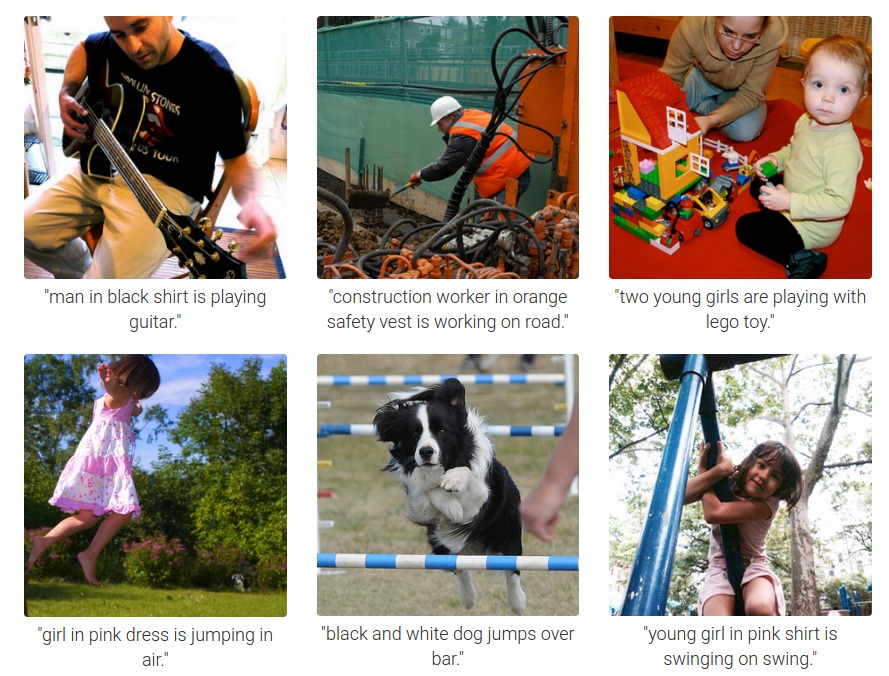
\includegraphics[width=\textwidth]{images/generated_descriptions.jpg}
\end{figure}
\end{frame}

\begin{frame}{Other topics}
\vfill
Machine learning is a wide and growing field. It also includes:	
\pause 
\vfill
\begin{itemize}
	\item Clustering (no predifined label/output)
\pause 
\vfill
	\item Dimensionality reduction
\pause 
\vfill
	\item \ldots
\end{itemize}
\vfill
\end{frame}

\begin{frame}{The course}
Goals:
\begin{itemize}
	\item Introduce \textbf{main concepts} of machine learning
	\item \textbf{Implement} these concepts in Python (Scikit-learn)
\end{itemize}
\vfill
\pause 
Practical information:
\begin{itemize}
	\item $\sim$ \textbf{10 90-min sessions}
	\item Alternating between \textbf{lectures and lab sessions}
	\item I will send you the slides + code after each course
\end{itemize}
\end{frame}

\begin{frame}{Course outline}
\vfill
\begin{itemize}
  \item \textbf{General introduction} to ML and Python (course + lab)
  \item \textbf{Regression} model (course + lab)
  \item \textbf{Classification} models (course + lab)
  \item \textbf{Clustering} models (course + lab)
  \item \textbf{Evaluation} methods
  \item \textbf{General conclusion} + questions + remarks and feedback
\end{itemize}
\vfill
\textbf{Note}: This is a first estimation. I will adapt to your needs.
\end{frame}

\begin{frame}{Python and Scikit-learn}
\vfill
Why Python?
\vfill
\begin{itemize}
	\item Intuitive, interpreted language
	\item Cross-platform (Windows, MacOS, Linux)
	\item An active open-source community
	\item Easy-to-use ML libraries (e.g. Scikit-learn)
\end{itemize}
\vfill
Let's see an example\ldots
\vfill
First lab session (about Python) next Thursday
\vfill
\end{frame}

\begin{frame}{Want to work on your own computer?}
\vfill
Recommended setup:
\vfill
\begin{itemize}
	\item \textbf{Anaconda} for Python \textbf{2.7}
	\newline \texttt{https://docs.continuum.io/anaconda/install}
\begin{center}
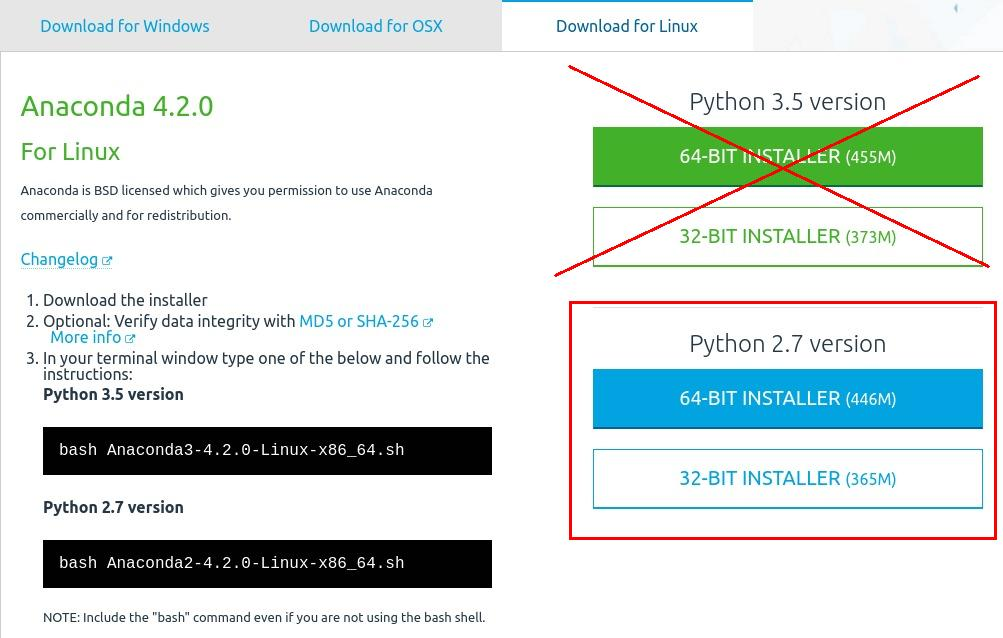
\includegraphics[width=0.75\textwidth]{images/anaconda_download.jpg}
\end{center}
	\item \textbf{Spyder} text editor
\end{itemize}
\vfill
\end{frame}

\begin{frame}
\vfill
\centering
\huge{Thank you! Questions?}
\vfill
Don't forget to send me an email: \texttt{alexis.zubiolo@gmail.com}
\vfill
\end{frame}

\end{document}
